\documentclass[english,11pt]{beamer}

\DeclareMathOperator{\Cov}{Cov}
\DeclareMathOperator{\Var}{Var}
\DeclareMathOperator{\E}{\mathbb{E}}
\DeclareMathOperator{\Proba}{\mathbb{P}}

\newcommand{\Covb}[2]{\ensuremath{\Cov\!\left[#1,#2\right]}}
\newcommand{\Eb}[1]{\ensuremath{\E\!\left[#1\right]}}
\newcommand{\Pb}[1]{\ensuremath{\Proba\!\left[#1\right]}}
\newcommand{\Varb}[1]{\ensuremath{\Var\!\left[#1\right]}}

% norm
\newcommand{\norm}[1]{\| #1 \|}

\newcommand{\indep}{\rotatebox[origin=c]{90}{$\models$}}





\usepackage{mathptmx,amsmath,amssymb,graphicx,bibentry,bbm,babel,ragged2e}

\makeatletter

\newcommand{\noun}[1]{\textsc{#1}}
\newcommand{\jitem}[1]{\item \begin{justify} #1 \end{justify} \vfill{}}
\newcommand{\sframe}[2]{\frame{\frametitle{#1} #2}}

\newenvironment{centercolumns}{\begin{columns}[c]}{\end{columns}}
%\newenvironment{jitem}{\begin{justify}\begin{itemize}}{\end{itemize}\end{justify}}

\usetheme{Warsaw}
\setbeamertemplate{footline}[text line]{}
\setbeamertemplate{headline}{}
\setbeamercolor{structure}{fg=purple!50!blue, bg=purple!50!blue}

\setbeamersize{text margin left=15pt,text margin right=15pt}

\setbeamercovered{transparent}


\@ifundefined{showcaptionsetup}{}{%
 \PassOptionsToPackage{caption=false}{subfig}}
\usepackage{subfig}

\usepackage[utf8]{inputenc}
\usepackage[T1]{fontenc}

\usepackage{multirow}

\usepackage{mdframed}


\makeatother

\begin{document}



\title{Construction of geo-commons by communities of practice: the case of orienteering maps generation from open LIDAR data}

\author{J.~Raimbault$^{1,2,3,4}$\\
\texttt{juste.raimbault@ign.fr}
}


\institute{$^{1}$LASTIG, Univ. Gustave Eiffel, IGN-ENSG\\
$^{2}$CASA, UCL\\
$^{3}$UPS CNRS 3611 ISC-PIF\\
$^{4}$UMR CNRS 8504 G{\'e}ographie-cit{\'e}s
}


\date{\textit{Journ{\'e}e de la Recherche UGE-IGN-ENSG 2024}\\
28/03/2023
}



\frame{\maketitle}

\sframe{Digital twins as commons?}{

More general framework of ``\textit{g{\'e}o-communs}'', launched by IGN since January 2021 \url{https://www.ign.fr/institut/la-demarche-geocommuns}.

\smallskip

\begin{center}

\includegraphics[width=0.15\linewidth]{figures/LOGO_IGN.png}
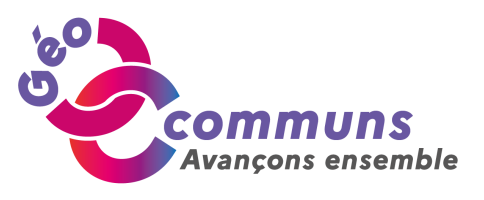
\includegraphics[width=0.54\linewidth]{figures/geocommuns.png}
\end{center}

\smallskip

$\rightarrow$ all IGN data is now open data 

$\rightarrow$ mutualisation, collaboration around tools, methods, databases

$\rightarrow$ public consultation in May 2021 (165 stakeholders from various backgrounds)

\medskip

\footnotesize

\textbf{Definition: } ``\textit{Geographic Information databases co-producted or co-maintained, and co-developped tools and methods, following an open common governance, to garantee a full appropriation by communities of users/producers/stakeholders/citizens}''

}

\sframe{Open questions for geocommons}{

\begin{enumerate}
	\item Governance of geocommons: mediator $\neq$ technical coordinator
	\item Economic model: public service (open public good)
	\item Core data: static digital twin at the national scale?
	\item Data production: e.g. link with OSM
	\item Licence: open licence but not ODbL?
	\item Methods and tools: ecosystem of open source softwares
	\item Open science as a part of geocommons
	\item Crucial role for environmental data
	\item Link with European directives for open data; European geocommons?
\end{enumerate}

}


\sframe{Research question}{


% ! def community of practice

%One important aspect of geo-commons lies in the diversity of their sourcing, and consequently in the possibility of crowdsourcing by domain experts in very specific contexts, enabled by the open sourcing of raw data, tools and methods. We propose in this contribution to illustrate such processes of geo-commons construction through the niche domain of orienteering maps generation from open LIDAR data.

$\rightarrow$ one core aspect of geo-commons is their diverse sourcing, applications and stakeholders

\medskip

$\rightarrow$ specific communities of practice involve niche knowledge experts, potentially rich for the construction of geo-commons, making it an interesting sociological field

\medskip

$\rightarrow$ orienteering map generation with LIDAR data is an example of such a niche community of practice


\bigskip
\bigskip


\textbf{Research question:}

\textit{What are the characteristics of communities using automatic orienteering map generation with LIDAR data, across different countries and contexts? How does this inform processes of geo-commons construction?}

$\rightarrow$ at this stage, preliminary qualitative analysis of stakeholders and contexts.

}


\sframe{Orienteering maps}{


% Forest orienteering maps have a large scale (1/10000 for middle distance and 1/15000 for long distance) and a quasi exhaustive description of topographic details, implying a very high production cost by expert cartographers. 

% ex bleau ancienne et recente!

Highly detailed topographic maps (mostly forest/natural areas), scale 1/10000 or 1/15000, high production cost and few mapping experts ; mapping norms by the IOF \cite{zentai2001development}

\bigskip

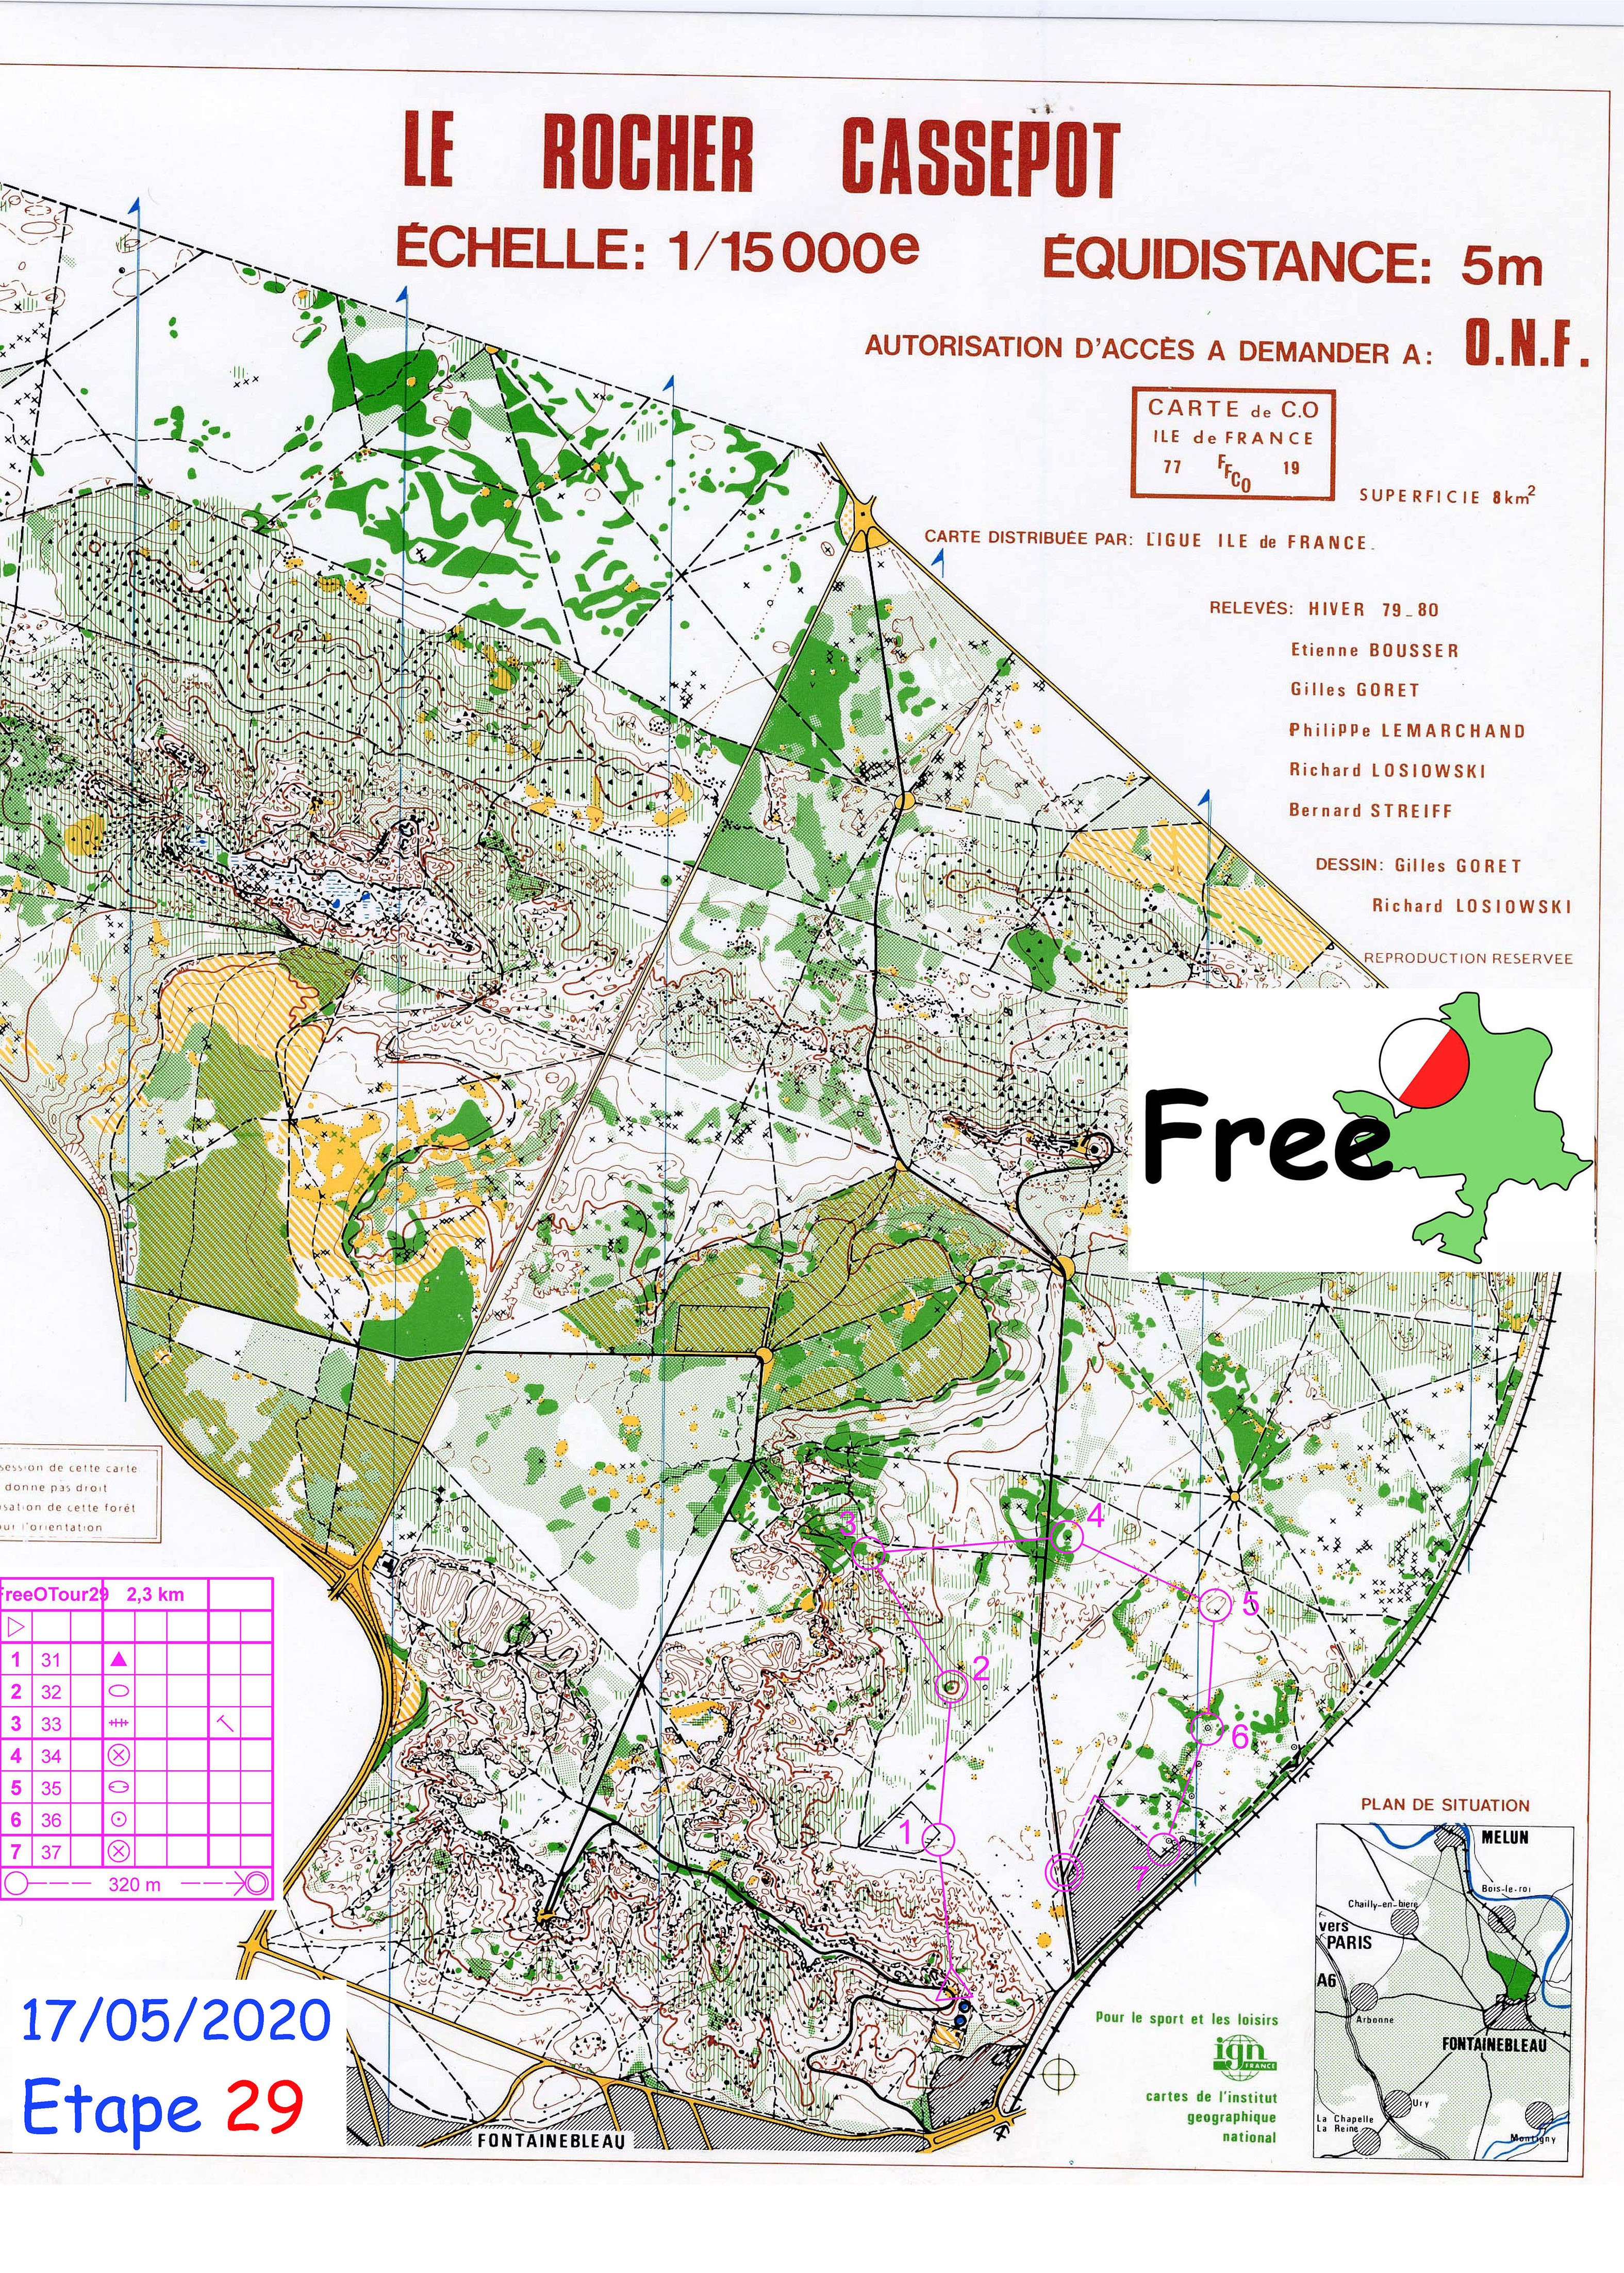
\includegraphics[width=0.4\linewidth]{figures/FreeOTour29_A4.jpg}\hspace{0.5cm}
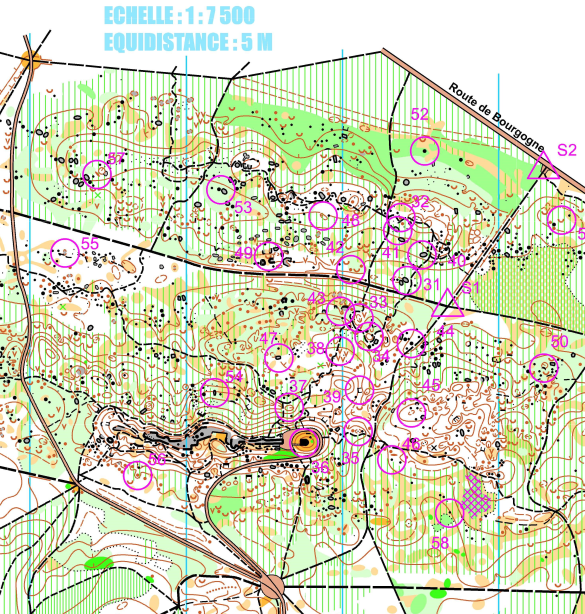
\includegraphics[width=0.5\linewidth]{figures/tour_denec.png}

}

\sframe{Map generation from LIDAR data}{

% Although the interpretation and selection part remains crucial and fieldwork still necessary, base map automatic generation from LIDAR data has shown a significant potential in reducing mapping costs and times, but also in empowering runners to train on previsouly unmapped terrains.

New technologies (GPS, LIDAR) have a significant potential in reducing costs and extending mapped coverage \cite{zentai2007new}

\bigskip

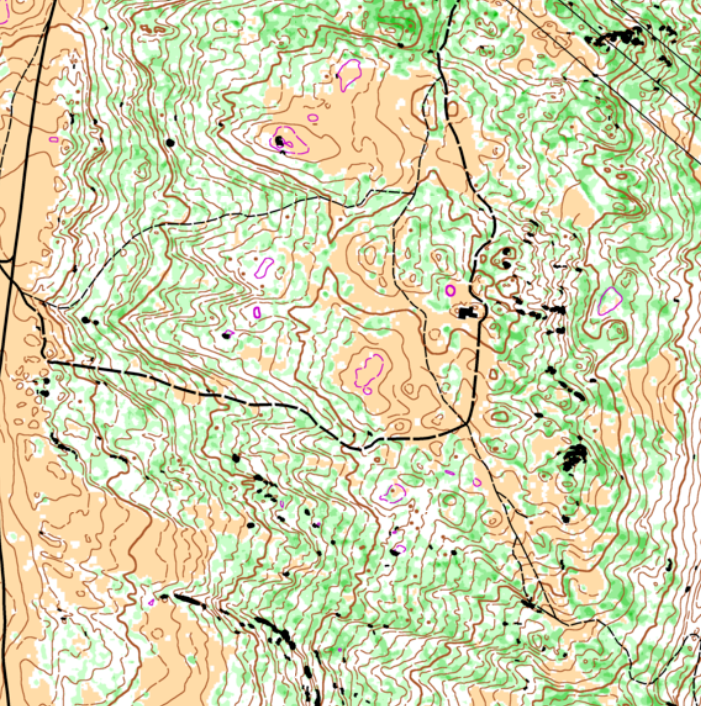
\includegraphics[width=0.45\linewidth]{figures/middle_lidar.png}\hspace{0.5cm}
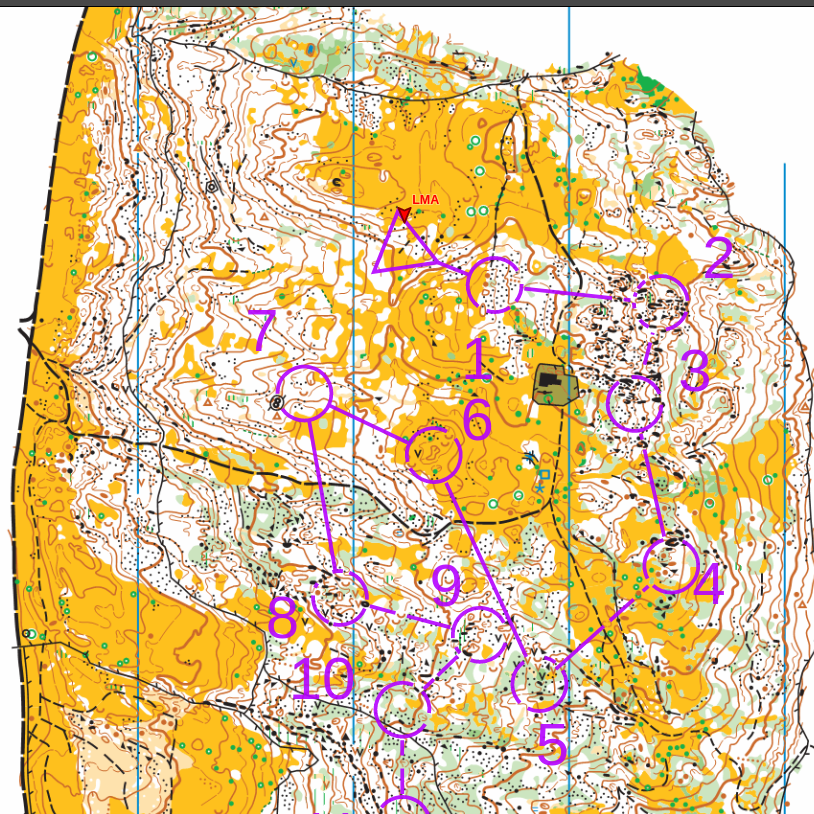
\includegraphics[width=0.45\linewidth]{figures/middle.png}

}

\sframe{Mapping coverage}{

High potential for outdoor activities: empower runners to discover new areas, avoid overcrowding, long-range projects, \ldots

\bigskip

% mention across Norway

\centering

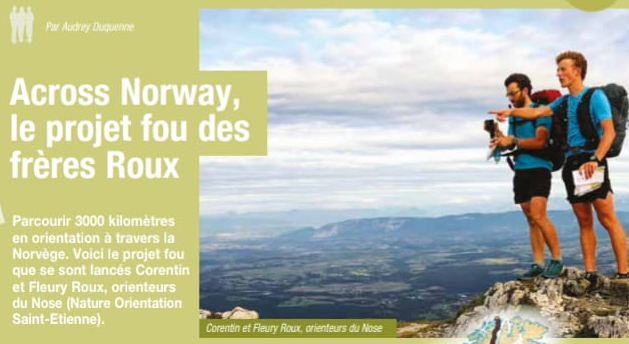
\includegraphics[width=0.7\linewidth]{figures/accrossnorway_1.png}
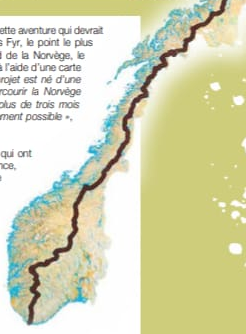
\includegraphics[width=0.29\linewidth]{figures/accrossnorway_2.png}

}



\sframe{The Mapant initiative}{




% The free software Karttapullautin has allowed communities of practice of orienteering mappers in several countries (Norway, Finland, Switzerland, France, Spain, New Zealand) to systematically generate maps accross an unprecendeted coverage.

Free software Karttapullautin to generate base maps from LIDAR data, open source forks also developped \url{https://github.com/rphlo/rusty-pullauta}

\medskip

Systematic processing in several countries with full LIDAR coverage: (Norway, Finland, Switzerland, France, Spain, New Zealand)

\medskip

\centering

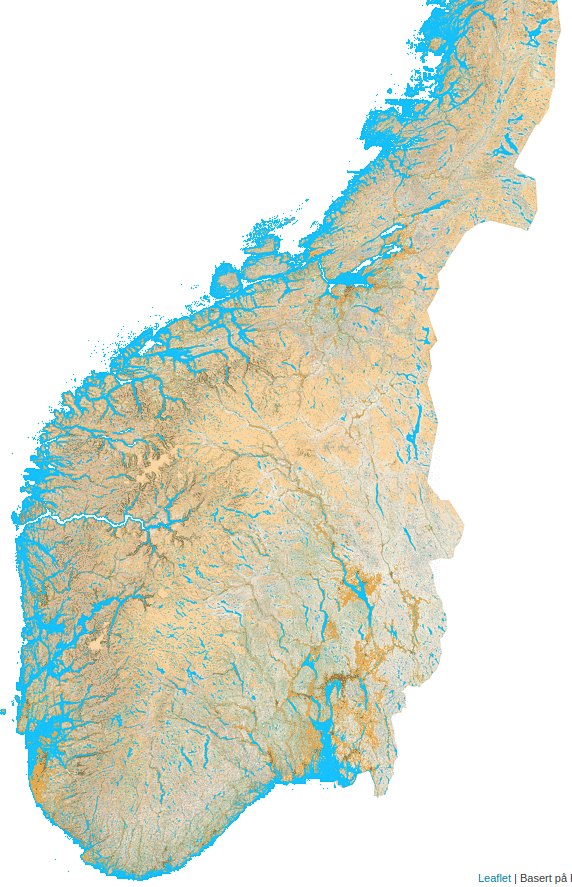
\includegraphics[width=0.25\linewidth]{figures/mapant_nor.png}\hspace{0.5cm}
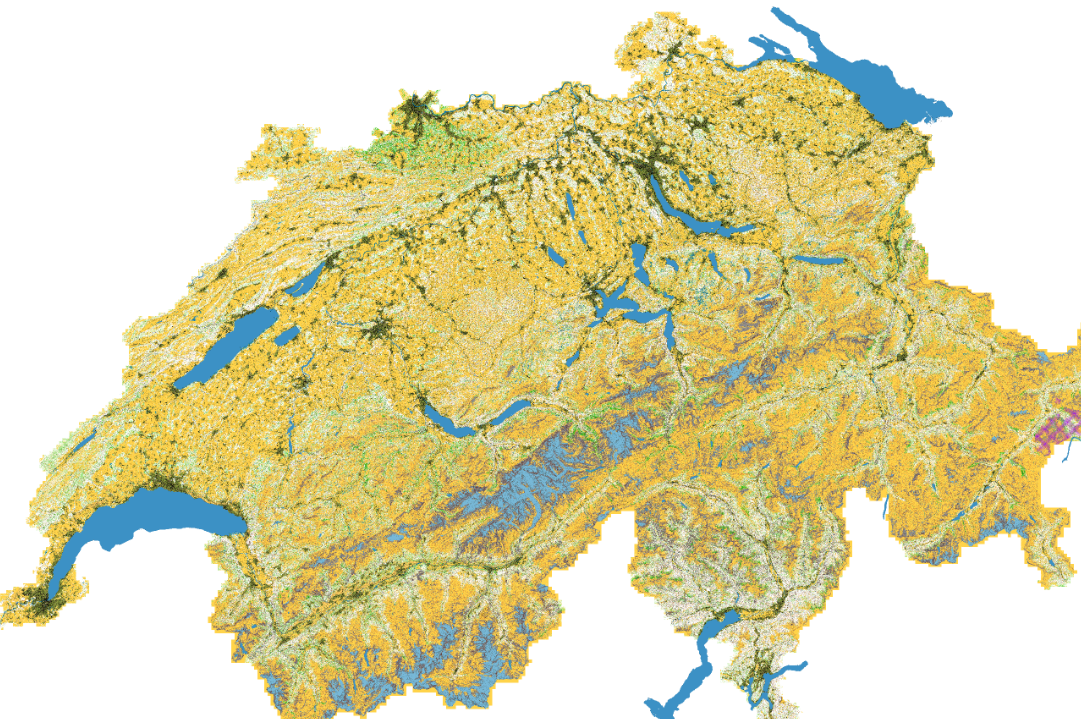
\includegraphics[width=0.35\linewidth]{figures/mapant_swi.png}\hspace{0.5cm}
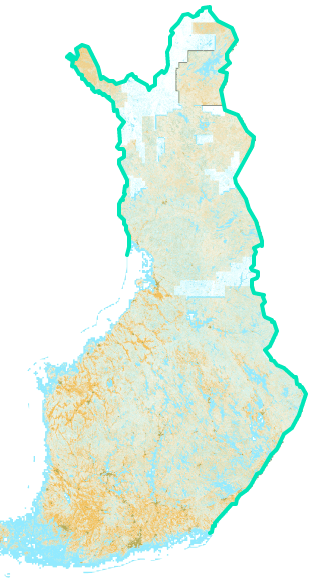
\includegraphics[width=0.2\linewidth]{figures/mapant_fi.png}


}

\sframe{The Mapant initiative}{

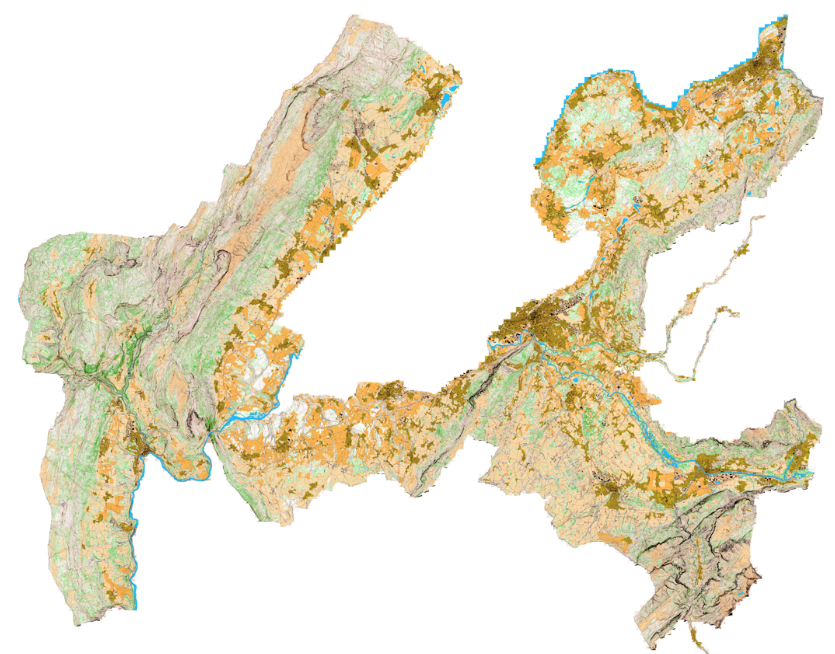
\includegraphics[width=0.35\linewidth]{figures/mapant_fr.png}\hspace{0.5cm}
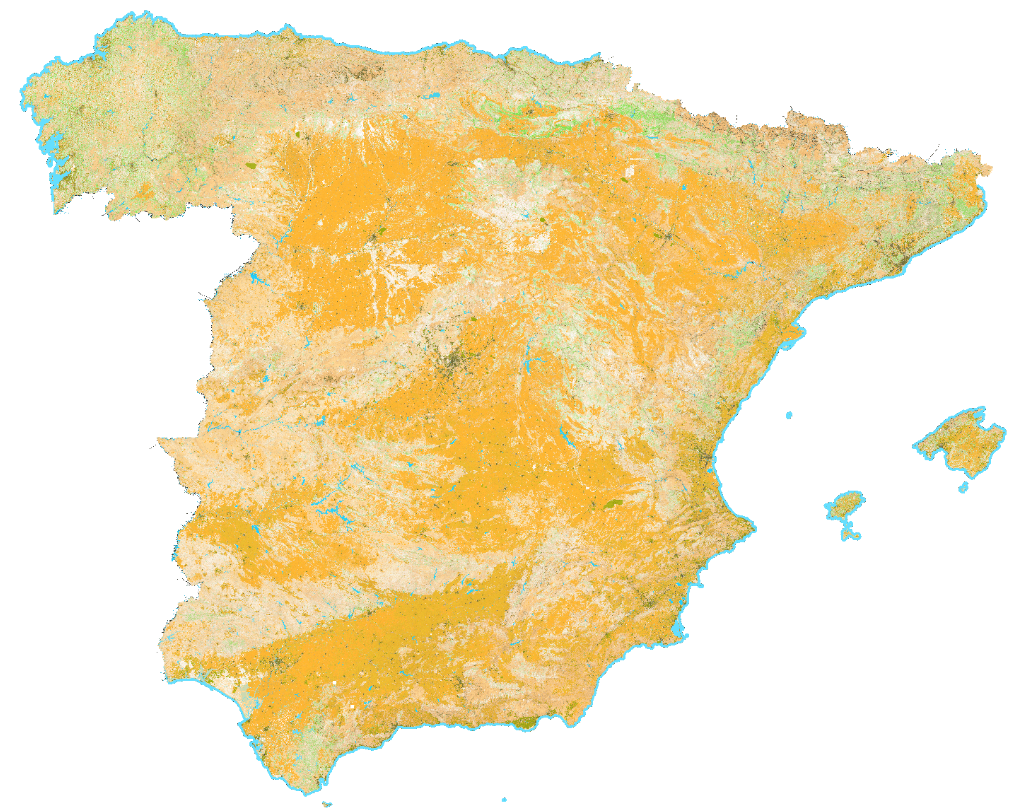
\includegraphics[width=0.35\linewidth]{figures/mapant_esp.png}\hspace{0.5cm}
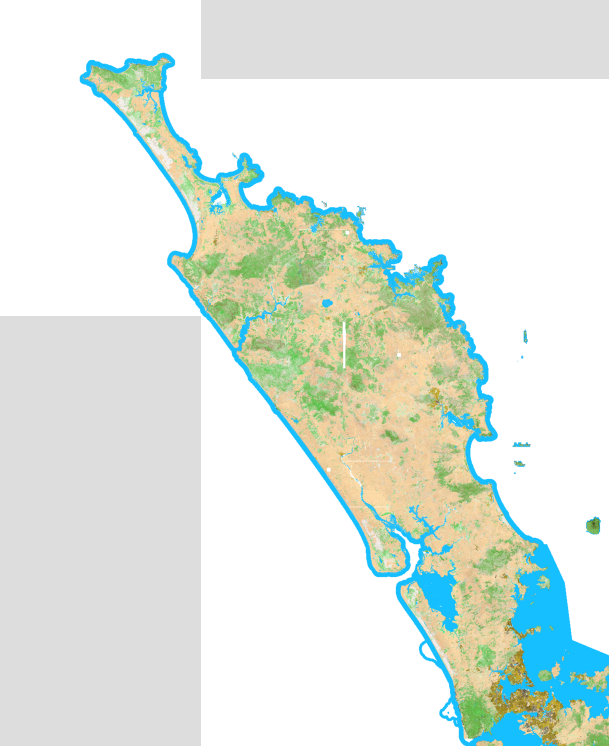
\includegraphics[width=0.18\linewidth]{figures/mapant_nz.png}

}


\sframe{Comparative analysis}{

% We detail the different production contexts, in which institutional or private partners can be involved.

% institutional context

% licence: data, generated maps

% coverage

% usage?
% TODO find way to informally collect maps, runners using it, ?

% TODO add data sources (OSM for some, not all?)

% TODO add tools / libraries

\tiny

\begin{center}
	\begin{tabular}{|p{1.7cm}|p{1.8cm}|p{1.4cm}|p{1.5cm}|p{1.5cm}|p{1.5cm}|}
	\hline
 Country & Institutional context & Data licence & Maps licence & Coverage & Usage \\\hline 
 Norway & Collab. State Mapping Agency / National Federation & CC-BY & CC-BY-NC & 62\% & Suggested for course planning \\ 
  Finland & Individuals & CC-BY & CC-BY & $\sim 80\%$ & Suggested as background map ; WMTS/WMS \\  
   Switzerland & Private company / local authorities / clubs & Various & NA & > 95\% & WMTS \\  
    France & Individuals & NA & NA & < 5\% & Elite athletes \\  
     Spain & Collab. State Mapping Agency / National Federation / Individuals & CC-BY/ODbL & CC-BY & > 95\% & NA \\  
      New Zealand & Individuals & CC-BY & NA & $\sim 50\%$ & WMTS \\\hline
	\end{tabular}
\end{center}


}


\sframe{Discussion}{


% Future work will include interviews with stakeholders in the various country contexts, to better understand stakes at play during the contruction of geo-commons.

\textbf{Results}

\medskip

$\rightarrow$ various stakeholders (institutional, collectivities, individuals), tools, licences, \ldots for mostly the same geo-common in terms of final data

\medskip

$\rightarrow$ which implications in terms of durability and accessibility? Which role of local usages in the initiative?



\bigskip


\textbf{Future work}

\medskip

$\rightarrow$ interviews with mappers, stakeholders, for a more detailed sociological study of production contexts

\medskip

$\rightarrow$ broad online survey of usages


}




%%%%%%%%%%%%%%%%%%%%%
\begin{frame}[allowframebreaks]
\frametitle{References}
\bibliographystyle{apalike}
\bibliography{biblio}
\end{frame}
%%%%%%%%%%%%%%%%%%%%%%%%%%%%






\end{document}



















